\documentclass[../main.tex]{subfiles}

\begin{document}
\chapter{Drivers of Antarctic Land Ice}
\label{chap:land_ice}
In chapter \ref{chap:temp_and_ice}, we found that temperature is significant for our understanding of the trends in Antarctic \gls{sic} over the last 40 years. However we found that the relationship between temperature and land ice is not as strong. To understand this we will have to do some more calculations.

We want to consider a range of variables which could be impacting land ice in Antarctica. We will include temperature again for completeness. Wind speed is linked to atmospheric circulations which move clouds and thermal energy around the continent. Cloud cover has also been linked to behaviours in the land ice. \todo{add appropriate citations here}. 

\section{Time-frame of datasets used in this chapter}
For this chapter we use a number of datasets, which each have data available for different time frames. Because of the limitations in table \ref{tab:landicedata} we will restrict our time-frame to 2014 - 2017.
% Please add the following required packages to your document preamble:
% \usepackage{booktabs}
\begin{table}[H]
\begin{tabular}{@{}lll@{}}
\toprule
Data                                     & Start Date   & End Date \\ \midrule
ECMWF ERA5 Reanalysis                    & January 1981 & Present  \\
GRACE \gls{lilwet}                       & August 2002  & 2017  \\
ARGO product \todo{check this} & January 2004 & Present  \\ \bottomrule
\end{tabular}
\caption{Different data sources used in this chapter.}
\label{tab:landicedata}
\end{table}

\section{Land ice trends and variability}
Before we start investigating what drives the changes in antarctic land ice, let's look again at the trends and behaviours seen in land ice specifically. We are interested in if the variables have impact on sea ice, however we have determined that sea ice trends and variability are largely driven by temperature, and so will not plot the trends and variability in sea ice again here.

The first plot to consider is the mean state of \gls{lilwet} (see Figure \ref{fig:lilwet_mean}).
 \begin{figure}[!hbt]
     \centering
     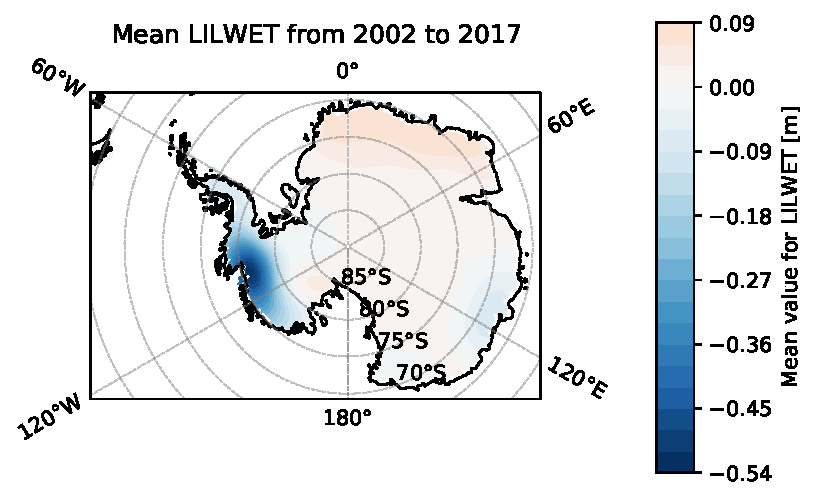
\includegraphics{images/2021w5/chapter7/hres/mean_spatial_LIC}
     \caption{Mean value of \gls{lilwet} from 2002 to 2017.}
     \label{fig:lilwet_mean}
 \end{figure}
 Looking at figure \ref{fig:lilwet_mean} we observe small values over most of the continent (maximum of 9 cm) whereas we have negative values of \gls{lilwet} over west Antarctica. The negative values are consequential of the way the data was measured (see Chapter \ref{chap:data} for more detail). The \gls{lilwet} data is anomalous from a baseline \todo{check what this baseline is}. This indicates that the \gls{wais} is a good place to focus our attention. For a better understanding of the behaviour of land ice let's look at the trend in \gls{lilwet} at each spatial gridpoint (see Figure \ref{fig:lilwet_trend}).
\begin{figure}[!hbt]
    \centering
    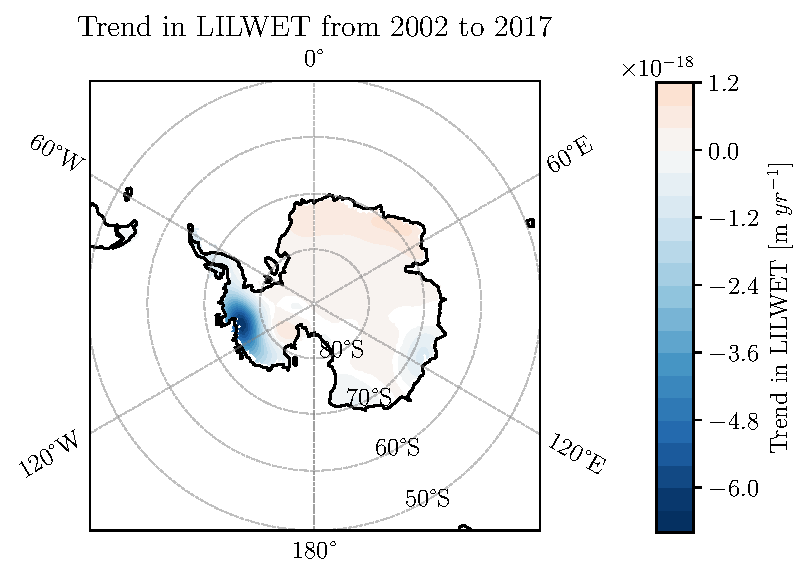
\includegraphics{images/2021w5/chapter7/hres/trend_spatial_LIC}
    \caption{Trend in Antarctic \gls{lilwet} from 2002 to 2007. Only statistically significant trends have been plotted, i.e. with a p-value $\leq$ 0.05.}
    \label{fig:lilwet_trend}
\end{figure}

Looking at figure \ref{fig:lilwet_trend} we can gain some understanding of how \gls{lilwet} changed from 2002 to 2007. This tells a similar story to what we saw in figure \ref{fig:lilwet_mean}, in that the \gls{wais} exhibits a large and significant decrease over time period. It is worth noting that while the trends over the rest of the continent and the \gls{eais} are small they are still statistically significant (with a p-value $\leq$ 0.05). This means that while we are mostly motivated to understand the strong decrease in the \gls{wais}, we cannot fully ignore the behaviour of ice in the \gls{eais}. Our final step before investigating the different variables which could impact the behaviour of Antarctic \gls{lilwet} is to look at the timeseries of mean Antarctic \gls{lilwet} from 2002 to 2017 (see Figure \ref{fig:lilwet_timeseries}).

\begin{figure}[!hbt]
    \centering
    \missingfigure{Plot of mean time-series of Antarctic ice}
    \caption{Time series of mean Antarctic \gls{lilwet} from 2002 to 2007.}
    \label{fig:lilwet_timeseries}
\end{figure}


The simplest thing we can do at this point is to compare the mean time series of this with different variables.

\section{Comparing land ice with different variables}
For the first step in analysis here we plotted the mean values for both land ice and other environmental variables, considering only the grid points where we have data for land ice.

\subsection{Trends in different variables}
We start by looking at the spatial pattern of trends in skin temperature (see Figure \ref{fig:trend_skt_02_17}).
\begin{figure}[!hbt]
    \centering
    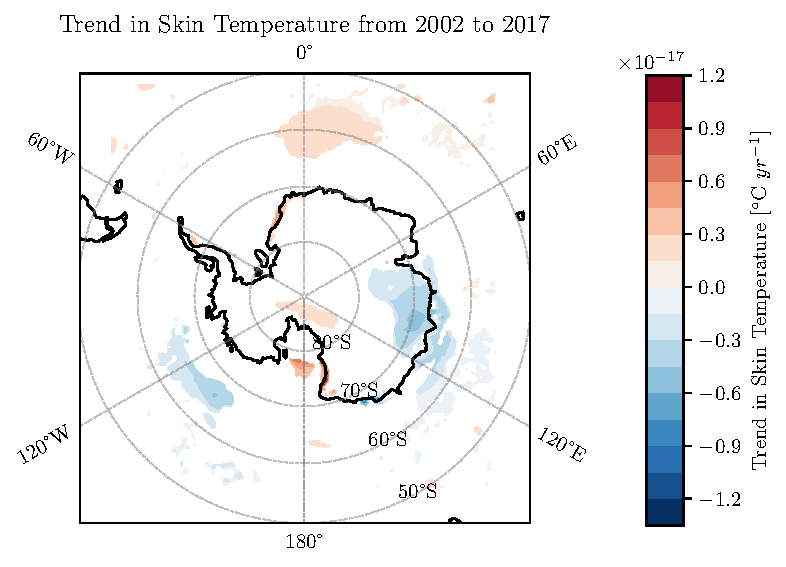
\includegraphics{images/2021w5/chapter7/hres/trend_spatial_skt}
    \caption{Trend in skin temperature over Antarctica from 2002 to 2017. Only statistically significant trends have been plotted, i.e. with a p-value $\leq$ 0.05.}
    \label{fig:trend_skt_02_17}
\end{figure}

Looking at the trend in skin temperature (figure \ref{fig:trend_skt_02_17}), we note that there is not a large region of the continent with statistically significant trends in skin temperature from 2002 to 2017. This is likely due to the large variability of temperature and the slowly moving trends. We can also look at the trends in subsurface oceanic temperatures (see Figure \ref{fig:trend_subsurtemp_02_17}) this is what has been predominantly proposed to have driven changes in Antarctic land ice by literature. The structure of the ocean and the temperature gradient is complicated and driven by a mixed layer close to the surface. To rigorously understand the relationship between land ice and oceanic temperatures, a condition for the depth of the mixed layer would have to be applied, \todo{add citation to paper from Melissa} however that is out of the scope of this thesis unless the results are exceptionally promising, which they are not. As a proxy for this we took the temperature at three different depths (100 dbar, 500 dbar, 700 dbar) and will be comparing these with the different ice variables. Our hope is that by considering a range of depths we will capture any physical processes occurring between land ice and subsurface temperatures without introducing more complicated considerations which would take more time to compute and introduce unnecessary errors in our results.
\begin{figure}[!hbt]
    \begin{subfigure}[b]{0.3\textwidth}
    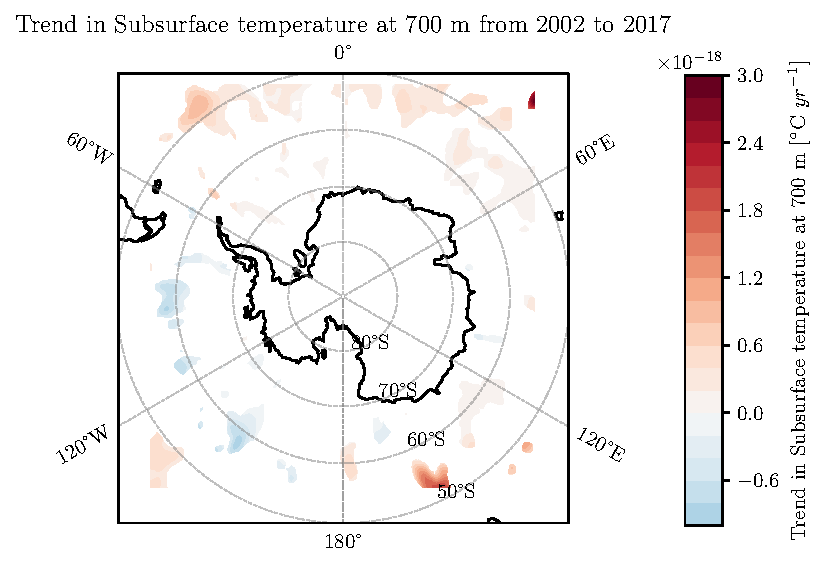
\includegraphics[width=\textwidth]{images/2021w5/chapter7/hres/trend_spatial_subsurtemp_700}
    \end{subfigure}
    \begin{subfigure}[b]{0.3\textwidth}
    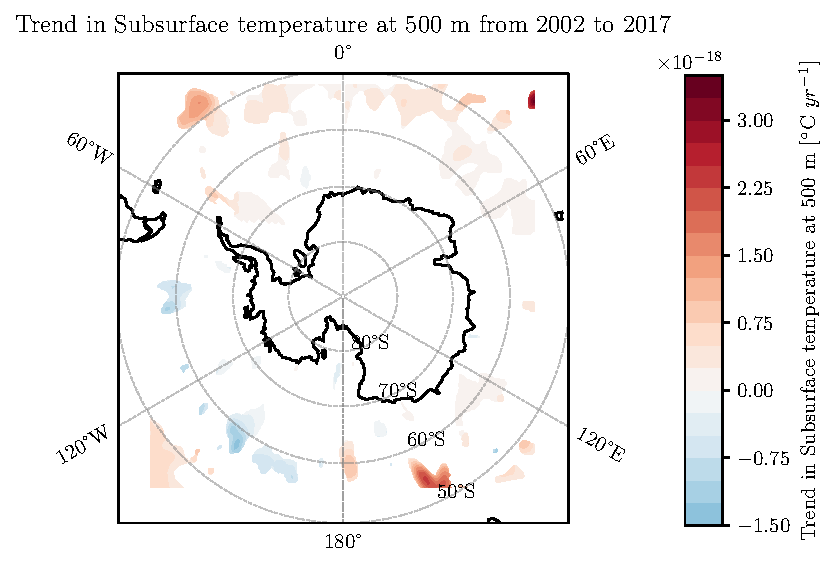
\includegraphics[width=\textwidth]{images/2021w5/chapter7/hres/trend_spatial_subsurtemp_500}
    \end{subfigure}
    \begin{subfigure}[b]{0.3\textwidth}
    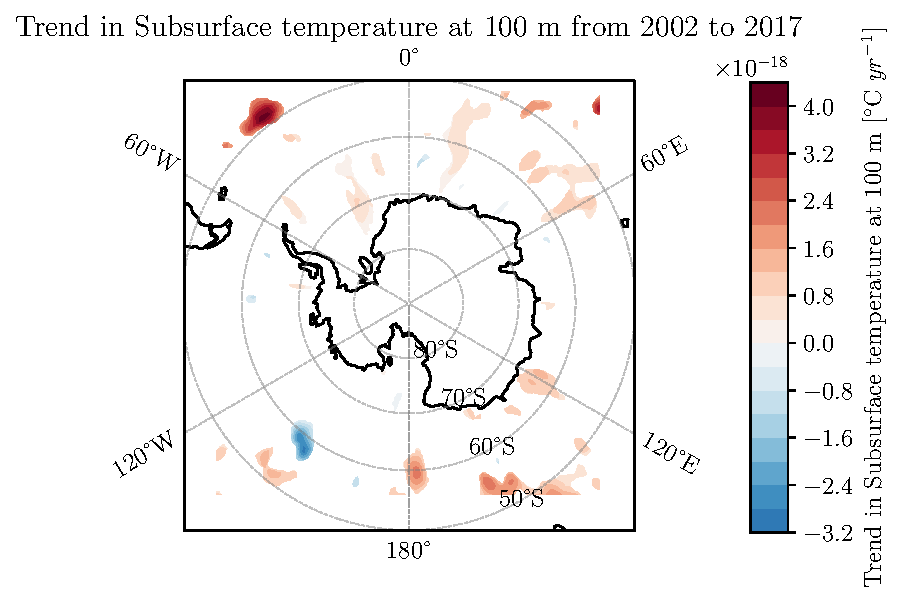
\includegraphics[width=\textwidth]{images/2021w5/chapter7/hres/trend_spatial_subsurtemp_100}
    \end{subfigure}
    \caption{Trend in subsurface oceanic temperature at different pressure levels over Antarctica from 2002 to 2017 \todo{make these sub-figures in python}. Only statistically significant trends have been plotted, i.e. with a p-value $\leq$ 0.05.}
    \label{fig:trend_subsurtemp_02_17}
\end{figure}

Looking at these sub-figures (figure \ref{fig:trend_subsurtemp_02_17}), we find like with skin temperature there are not many regions or a dominant pattern with a statistically significant trend in subsurface ocean temperatures at 100 dbar, 500 dbar or 700 dbar. 

We also want to consider the concentration of Ozone in the atmosphere at different levels. In literature this has been previously linked with land ice concentration change. \todo{cite this}. As such we consider the trend in ozone at different pressure levels. This data was sourced from the ERA5 reanalysis provided by ECMWF. We consider ozone mass mixing ratios at the same levels as other variables stratified \todo{check that I use stratified correctly} in the same manner, at 700 hPa, 500 hPa, and 200 hPa. We also want to consider what happens in the stratosphere as we know that ozone has been particularly dynamic there. So we also look at ozone mass mixing ratios at 100 hPa and 50 hPa. (See Figure \ref{fig:trend_o3_02_17}).

\begin{figure}[!hbt]
    \begin{subfigure}[b]{0.5\textwidth}
    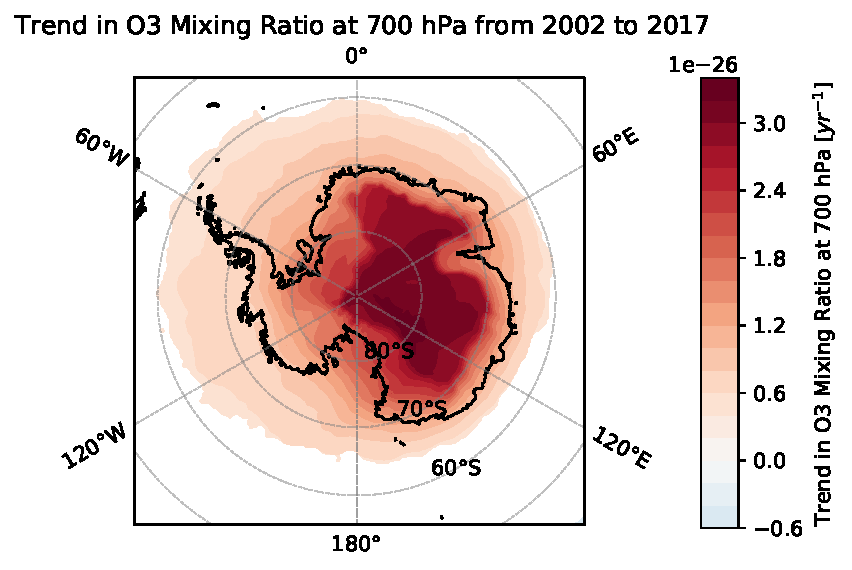
\includegraphics[width=\textwidth]{images/2021w5/chapter7/hres/trend_spatial_o3_700}
    \end{subfigure}
    \begin{subfigure}[b]{0.5\textwidth}
    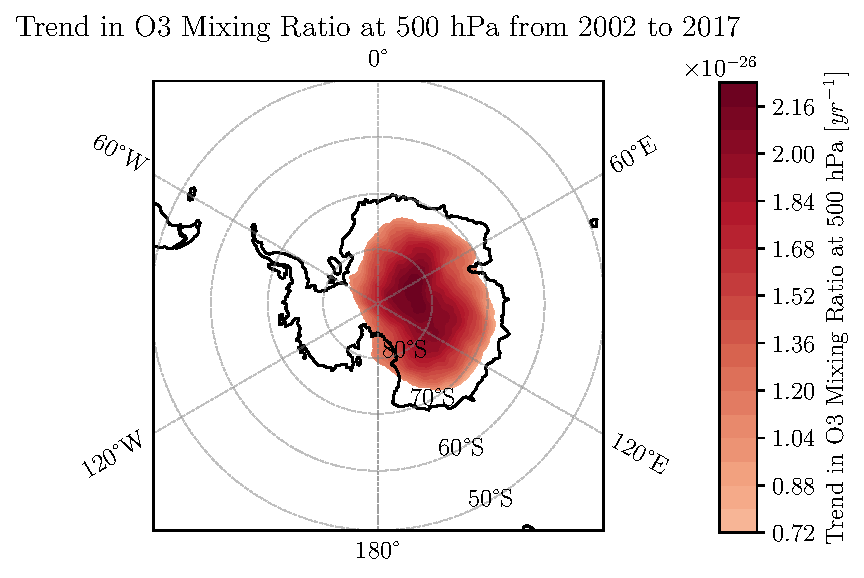
\includegraphics[width=\textwidth]{images/2021w5/chapter7/hres/trend_spatial_o3_500}
    \end{subfigure}
    \begin{subfigure}[b]{0.5\textwidth}
    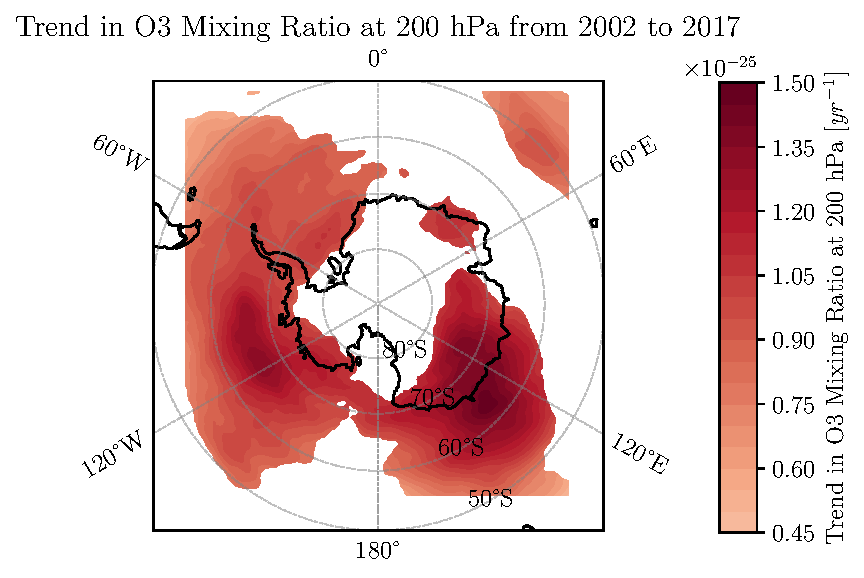
\includegraphics[width=\textwidth]{images/2021w5/chapter7/hres/trend_spatial_o3_200}
    \end{subfigure}
    \begin{subfigure}[b]{0.5\textwidth}
    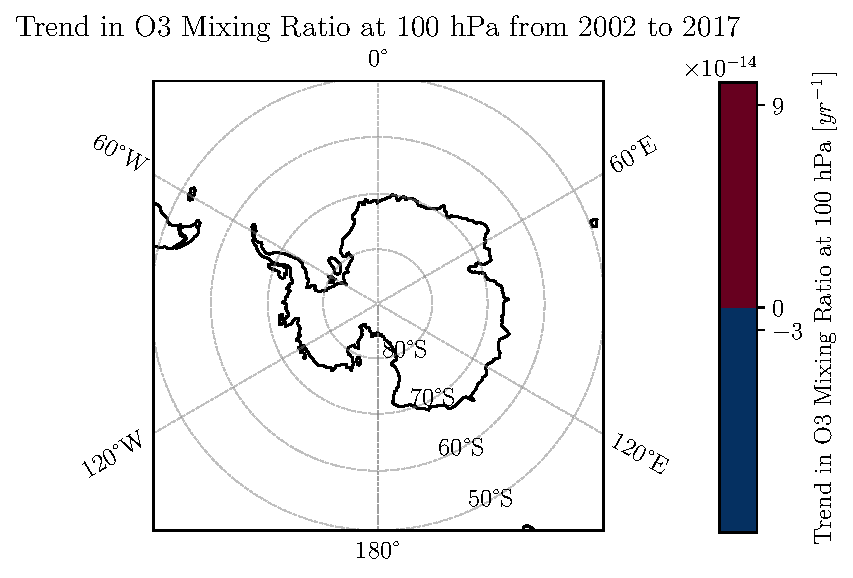
\includegraphics[width=\textwidth]{images/2021w5/chapter7/hres/trend_spatial_o3_100}
    \end{subfigure}
    \begin{subfigure}[b]{0.5\textwidth}
    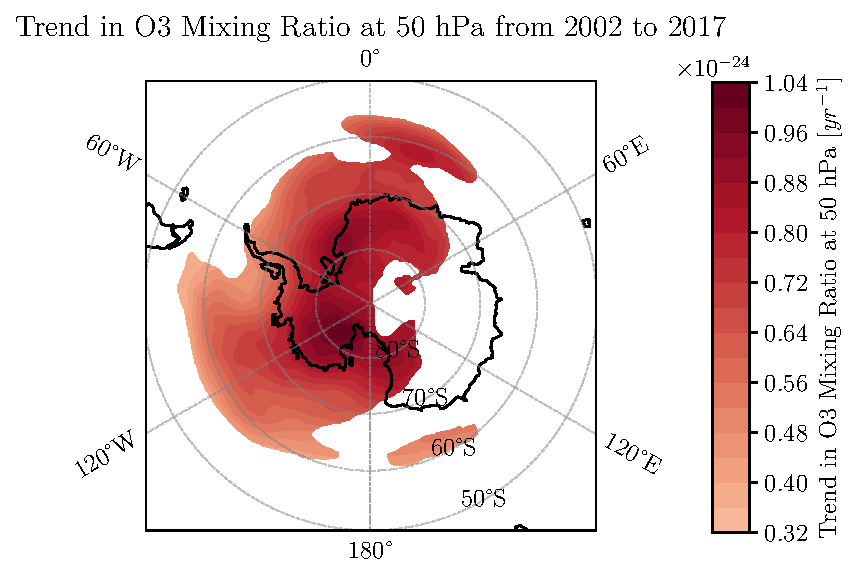
\includegraphics[width=\textwidth]{images/2021w5/chapter7/hres/trend_spatial_o3_50}
    \end{subfigure}
    \caption{Trend in ozone at different pressure levels over Antarctica from 2002 to 2017 \todo{make these sub-figures in python}. Only statistically significant trends have been plotted, i.e. with a p-value $\leq$ 0.05.}
    \label{fig:trend_o3_02_17}
\end{figure}

Looking at these plots we can make a couple observations. The ozone hole which has existed over Antarctica and has been disappearing over the last few decades. This is observed as a significant increase in ozone mass mixing ratio consistently over the entire continent at most pressure levels. We should note that no location has a significant trend for ozone at 100 hPa. At this level we do see some insignificant decreases in ozone.\todo{see if we know why this is the case or can find out quickly}

\missingfigure{Plot of trend wind speed}

\subsection{Visual time series comparison}
Now we have some understanding of the spatial distribution of trends in each variable we also want to consider how they change over time and how that compares to the mean \gls{lilwet}. We do this by taking the average value for each variable over Antarctica. Only computing the average with locations where we have access to land ice data. We want to acknowledge before including these plots, that these plots represent a large region of spatial variability and as such should be used only as general indicators in the context of understanding the behaviour of the different variables. Nonetheless useful information can still be obtained here. We start by plotting the time series for mean skin temperature over land and mean \gls{lilwet} (see figure \ref{fig:timeseries_skt}).

\begin{figure}[!hbt]
    \centering
    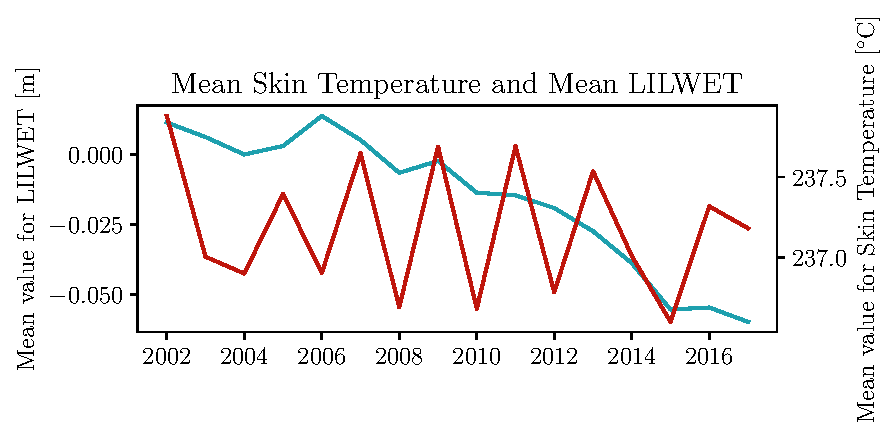
\includegraphics{images/2021w5/chapter7/hres/tiemseries_skt_LIC}
    \caption{Time-series of mean \gls{lilwet} and mean skin temperature over Antarctica. Mean is taken only over land.}
    \label{fig:timeseries_skt}
\end{figure}\todo{write up figure notes}
\begin{figure}[!hbt]
    \centering
    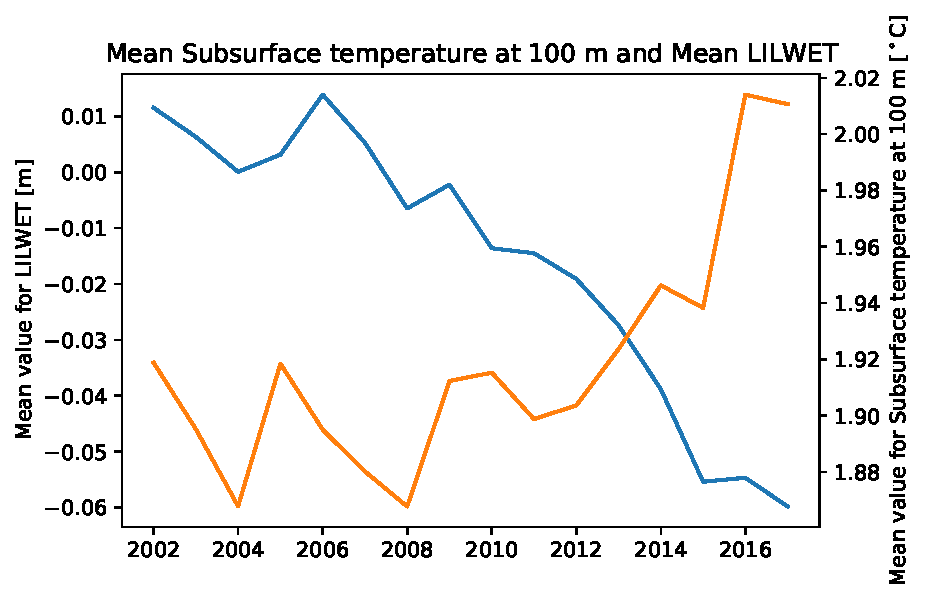
\includegraphics{images/2021w5/chapter7/hres/tiemseries_subsurtemp_100}
    \caption{Time-series of mean \gls{lilwet} and mean skin temperature over Antarctica. Mean is taken only over land.}
    \label{fig:timeseries_subsurtemp_100}
\end{figure}\todo{write up figure notes}
\begin{figure}[!hbt]
    \centering
    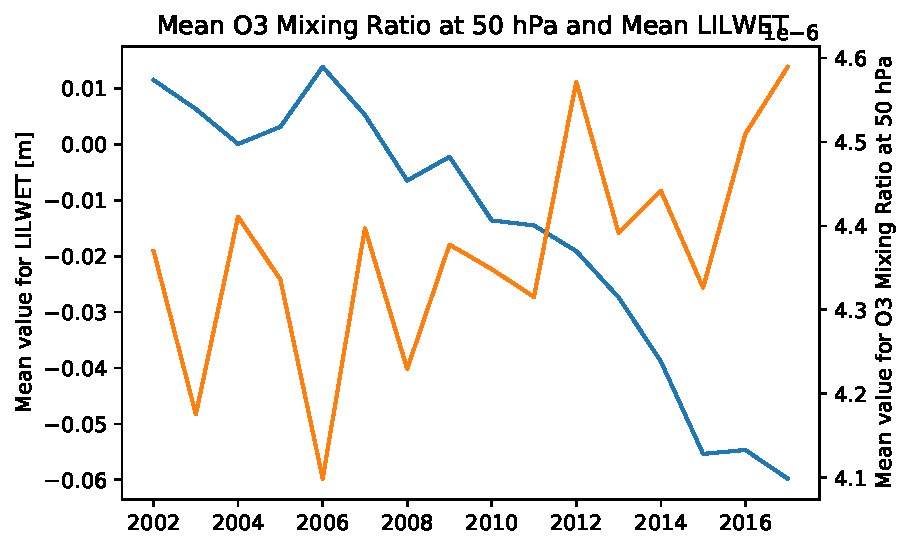
\includegraphics{images/2021w5/chapter7/hres/tiemseries_o3_50}
    \caption{Time-series of mean \gls{lilwet} and mean skin temperature over Antarctica. Mean is taken only over land.}
    \label{fig:timeseries_o3_50}
\end{figure}\todo{write up figure notes}\todo{add all pressure levels to single plot.}
\begin{figure}[!hbt]
    \centering
    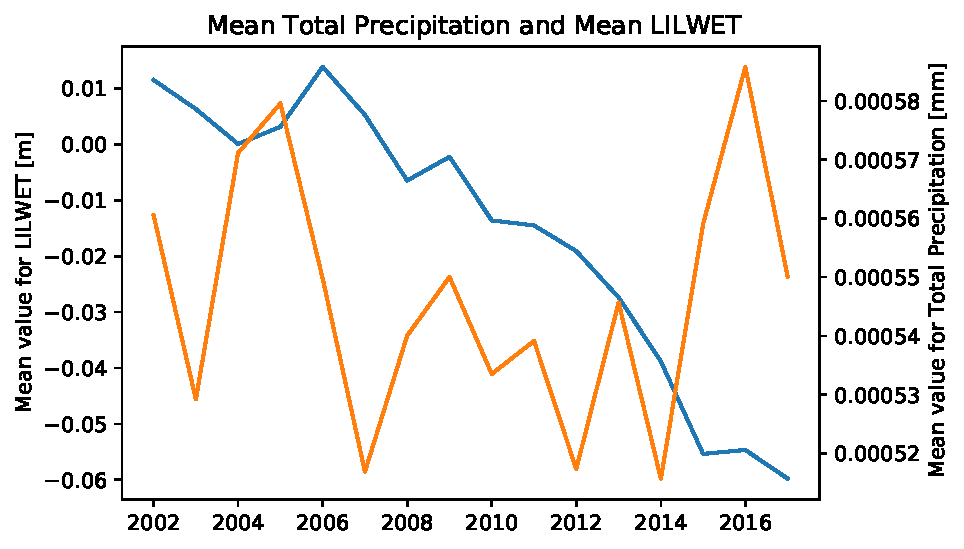
\includegraphics{images/2021w5/chapter7/hres/tiemseries_tp}
    \caption{Time-series of mean \gls{lilwet} and mean skin temperature over Antarctica. Mean is taken only over land.}
    \label{fig:timeseries_tp}
\end{figure}\todo{write up figure notes}
\begin{figure}[!hbt]
    \centering
    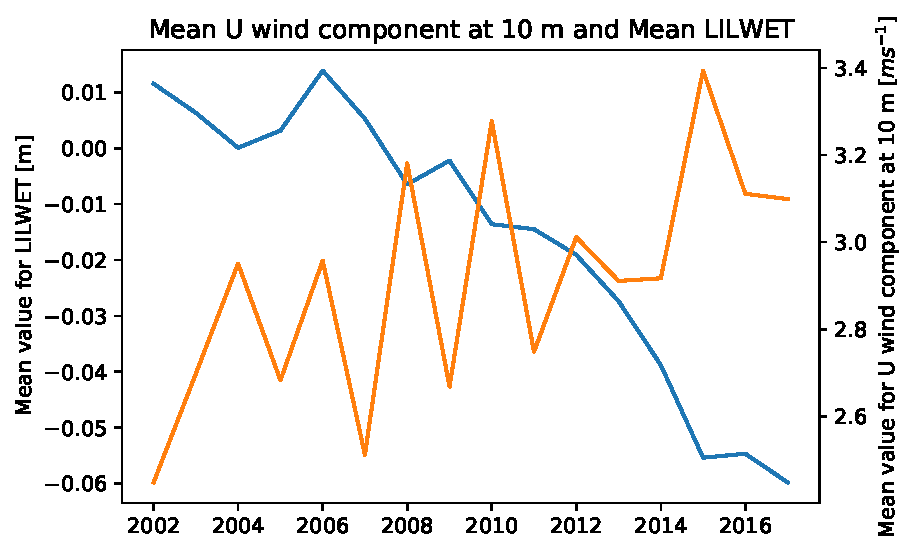
\includegraphics{images/2021w5/chapter7/hres/tiemseries_u_10}
    \caption{Time-series of mean \gls{lilwet} and mean wind speed over Antarctica. Mean is taken only over land.}
    \label{fig:timeseries_u_10}
\end{figure}\todo{write up figure notes}\todo{do total wind speed for this plot at different levels}

\subsection{Co-spatial Correlations}
Now we have some understanding of the way different variables behave over both time and space we can look at their correlations with Antarctic \gls{lilwet}. We will present all the results and discuss what we can learn from each one.

\begin{figure}[!hbt]
    \centering
    \missingfigure{correlation between skt and ice}
    \caption{Caption}
    \label{fig:my_label}
\end{figure}
\begin{figure}[!hbt]
    \centering
    \missingfigure{correlation between subsurtemp and ice}
    \caption{Caption}
    \label{fig:my_label}
\end{figure}
\begin{figure}[!hbt]
    \centering
    \missingfigure{correlation between o3 and ice}
    \caption{Caption}
    \label{fig:my_label}
\end{figure}
\begin{figure}[!hbt]
    \centering
    \missingfigure{correlation between tp and ice}
    \caption{Caption}
    \label{fig:my_label}
\end{figure}
\begin{figure}[!hbt]
    \centering
    \missingfigure{correlation between wind speed and ice}
    \caption{Caption}
    \label{fig:my_label}
\end{figure}

\section{Identifying drivers for significant decrease}

\subsection{Identifying region with significant decrease}

\subsection{Spatial correlations}

\subsection{Regressions}

\section{Discussion and implications of these results}

\end{document}